%%%%%%%%%%%%%%%%%%%%%%%%%%%%%%%%%%%%%%%%%%%%%%%%%%%%%%%%%%%%%%%%%%%%%%%%%%%
%%
%%  ap-programs.tex
%%
%%  Created: Fri Oct 10 14:24:37 1997
%%  Author.: Jose Carlos Gonzalez
%%  Notes..:
%%          
%%-------------------------------------------------------------------------
%% Filename: $RCSfile$
%% Revision: $Revision$
%% Date:     $Date$
%%%%%%%%%%%%%%%%%%%%%%%%%%%%%%%%%%%%%%%%%%%%%%%%%%%%%%%%%%%%%%%%%%%%%%%%%%%


\chapter{Technical description of the programs for the analysis of 
  \MC data}
\label{appendix:programs}

The program and mode of operation for the generation of \MC data
(cosmic ray and gamma ray initiated atmospheric showers) has been
described in Chapter \ref{chapter:simshowers} and Appendix
\ref{appendix:corsika}, while the programs created for the analysis of
these \MC data were mentioned, and its behavior explained, in Chapter
\ref{chapter:simmagic}. Here, we will talk about the technicalities
and the usage of these later programs.

\afterpage{\clearpage}


\section{Definition of the Telescope}
\label{sec:ctdef}

There are two main programs developed for such task: \reflector and
\camera. The first one tries to simulate the mirrors, frame and
optical characteristics of \MAGIC, while the second tries to simulate
the camera of \MAGIC. Actually, this is not rigorously true: both
codes get as part of their input what is called a \emph{CT definition
  file}. This file has a list of parameters in the form 
%
\begin{verbatim}
   <keyword>   [ <value1> [ <value2> ... ] ]
\end{verbatim}
%
Lines starting with the character ``\texttt{\#}'' are treated as
comment lines, and ignored. The keywords currently supported (i.e.,
understood by \reflector) are shown in Table \ref{tbl:ctdefkeywords}.
The units, when needed, are the typical ones used in \CORSIKA, namely
$[L]=\u{cm}$, $[T]=\u{s}$, $[E]=\u{GeV}$, and radians for the angles.
The first keyword must be \texttt{type}, since depending on its value
some of the other keywords get different meanings. The currently
available values for \texttt{type} are:
%
\begin{description}
\item[\texttt{type 0} :] for the first HEGRA telescope, \CTuno, and
\item[\texttt{type 1} :] for the \MAGIC telescope
\end{description}
%
Most of the keywords get a number as a parameter, while few of them
get more than one (like \texttt{n\_pixels} for \MAGIC, where one can
specify the number of pixels in the inner and outer part of the
camera, as well as the number gap pixels\footnote{It is possible that
  these gap pixels dissappear in the actual camera of \MAGIC. However,
  they were included in the first designs, and that's why they are
  used in the simulation.}). The last keyword,
\texttt{define\_mirrors}, needs no additional parameters: it acts as a
mark to let the program know where the actual definition of the
individual mirrors starts. After the line with the keyword
\texttt{define\_mirrors}, there appear a single line per mirror, with
a 12 numbers that fix the focal length, position and orientation of
that mirror in the frame of the telescope. The interpretation of these
numbers is different in general for \MAGIC and \CTuno, as shown in
Tables \ref{tbl:mirrordefCTuno} and \ref{tbl:mirrordefMAGIC}.

\ctdefkeywordstbl

\mirrordefCTunotbl

\mirrordefMAGICtbl

Some of the keywords (and their associated parameters) are redundant,
and are used for cross-checking only. This is the case of the keywords
\texttt{n\_pixels} and \texttt{n\_rings}, for a \MAGIC definition
file. These entries have the form
%
\begin{verbatim}
   n_pixels   A  B  C
   n_rings    P  Q  
\end{verbatim}
%
where \texttt{A}, \texttt{B}, \texttt{C}, \texttt{P} and \texttt{Q}
are integer numbers. This numbers are (see Fig. \fullref{fig:MAGICcamera}, Chapter \ref{fig:MAGICcamera}):\\
%
\begin{center}
\begin{tabular}{cl}
\texttt{A} & Number of ``inner'' pixels (in the central region of
  the camera)\\
\texttt{B} & Number of ``gap'' pixels \\
\texttt{C} & Number of ``outer'' pixels (in the external region of
  the camera)\\
\texttt{P} & Number of ``rings'' of pixels in the central region of 
  the camera\\
\texttt{Q} & Number of ``rings'' of pixels in the external region of 
  the camera\\
\end{tabular}
\end{center}
%
If we define the value $n$ as the \emph{number of outer pixels in the
  first row of a segment of the camera}, $ n \equiv
\mathcal{E}[(\texttt{A}+1)/2]$ (with $\mathcal{E}[\mathord{.}]$ being
the ``integer part'' function), then we have:
%
\calcnpixelseq

Finally, the interpretation of the values associated to some keywords
is different in the case of \MAGIC and \CTuno. For example,
\texttt{r\_mirrors} contains the radius of the circular mirrors in the
case of \CTuno, while the value for \MAGIC is interpreted as the
shortest distance from the center of the square mirrors to one of
their edges.

%\begin{figure}[htbp]
%  \centering
%  \tiny
%  \hrule width \textwidth depth .01pt \vskip 5pt
%  \begin{verbatim}
%###################################################-*-sh-*-##
%# MAGIC definition file
%#############################################################
%# @file         magic.definition
%# @title        MAGIC definition file
%# @description  MAGIC def. file to be used by |reflector| and |camera|
%# @author       J C Gonzalez
%# @email        gonzalez@mppmu.mpg.de
%#
%# @maintitle
%# @code
%#------------------------------------------------------------ 
%# MAGIC definition file
%#------------------------------------------------------------
%#
%#---- type of definition file  (0: CT1, 1: MAGIC)
%type  1
%#
%#---- focal distance [cm]
%focal_distance      1700.0
%#
%#---- std(focal_distance) [cm]
%focal_std           0.0
%#
%#---- point spread function [cm]
%point_spread        0.5
%#
%# std(point spread function) [cm]
%#
%point_std           0.5
%#
%#---- std value of adjustment deviation [cm]
%adjustment_dev      0.5
%#
%#---- black spot in the center of the mirror, radius [cm]
%black_spot          0.5
%#
%#---- camera width [cm]
%camera_width        1000.
%#
%#---- number of pixels in the camera 
%#  INNER PIXELS = 3 x N x (N+1) + 1      (N=number of rings)
%#  OUTER PIXELS = 6 x (n + (n+1) + ... + (n+o)) (n=pix 1st segment; o=n.rings)
%#  GAP PIXELS   = 6 x (o-1)
%n_pixels  397 18 180 
%#
%#---- number of rings (inner region and outer region)
%n_rings 11 4 
%#
%#---- pixel width (small diameter) [cm] 
%pixel_width 3.0
%#
%#---- number of mirrors
%n_mirrors 920
%#
%#---- radius of a single mirror
%r_mirror 24.75
%#
%#---- this entry is followed by the def. of pixels, everything in [radians] or [cm]
%define_mirrors
%  1  1805.4000  -825.0000  -325.0000  -817.1337  -324.5073   113.6783   0.25348800   3.51962137   0.23307531   0.09256091   0.96804357
%  2  1805.4000  -825.0000  -275.0000  -817.1337  -274.7011   109.2895   0.24874869   3.46589971   0.23335783   0.07844938   0.96922123
%...     ...        ...        ...        ...        ...        ...        ...          ...          ...          ...          ...
%920  1805.4000   825.0000   325.0000   817.1337   324.5073   113.6783   0.25348800   0.37802872  -0.23307531  -0.09256091   0.96804357
%#@endcode
%#
%#EOF
%  \end{verbatim}
%  \hrule width \textwidth depth .01pt
%  \figcaption{Portion of a sample CT definition file (in this case, 
%    \texttt{magic.definition}).}
%  \label{fig:magicdef}
%\end{figure}

\begin{listado}
  \tiny
\begin{verbatim}

###################################################-*-sh-*-##
# MAGIC definition file
#############################################################
# @file         magic.definition
# @title        MAGIC definition file
# @description  MAGIC def. file to be used by |reflector| and |camera|
# @author       J C Gonzalez
# @email        gonzalez@mppmu.mpg.de
#
# @maintitle
# @code
#------------------------------------------------------------ 
# MAGIC definition file
#------------------------------------------------------------
#
#---- type of definition file  (0: CT1, 1: MAGIC)
type  1
#
#---- focal distance [cm]
focal_distance      1700.0
#
#---- std(focal_distance) [cm]
focal_std           0.0
#
#---- point spread function [cm]
point_spread        0.5
#
# std(point spread function) [cm]
#
point_std           0.5
#
#---- std value of adjustment deviation [cm]
adjustment_dev      0.5
#
#---- black spot in the center of the mirror, radius [cm]
black_spot          0.5
#
#---- camera width [cm]
camera_width        1000.
#
#---- number of pixels in the camera 
#  INNER PIXELS = 3 x N x (N+1) + 1      (N=number of rings)
#  OUTER PIXELS = 6 x (n + (n+1) + ... + (n+o)) (n=pix 1st segment; o=n.rings)
#  GAP PIXELS   = 6 x (o-1)
n_pixels  397 18 180 
#
#---- number of rings (inner region and outer region)
n_rings 11 4 
#
#---- pixel width (small diameter) [cm] 
pixel_width 3.0
#
#---- number of mirrors
n_mirrors 920
#
#---- radius of a single mirror
r_mirror 24.75
#
#---- this entry is followed by the def. of pixels, everything in [radians] or [cm]
define_mirrors
  1  1805.4000  -825.0000  -325.0000  -817.1337  -324.5073   113.6783   0.25348800   3.51962137   0.23307531   0.09256091   0.96804357
  2  1805.4000  -825.0000  -275.0000  -817.1337  -274.7011   109.2895   0.24874869   3.46589971   0.23335783   0.07844938   0.96922123
...     ...        ...        ...        ...        ...        ...        ...          ...          ...          ...          ...
920  1805.4000   825.0000   325.0000   817.1337   324.5073   113.6783   0.25348800   0.37802872  -0.23307531  -0.09256091   0.96804357
#@endcode
#
#EOF
\end{verbatim}
  \caption{Portion of a sample CT definition file (in this case, 
    \texttt{magic.definition}).}
  \label{fig:magicdef}
\end{listado}

A portion of one of the definition files used for \MAGIC is
shown\footnote{The words appearing there starting with a
  ``\texttt{@}'', are interpreted by a documentation system developed
  by the author, and are not needed for the normal operation of
  \reflector --- as one can see, they appear in comment lines.} in
Fig. \ref{fig:magicdef}. 

\afterpage{\clearpage}

\clearpage

\section{The code \reflector}
\label{sec:reflector}
%
The program that reads in the simulated atmospheric showers generated
by \CORSIKA is \reflector. This program takes as input a parameters
file, where the user specifies what showers to read and the set-up of
the telescope for their detection. Again, the parameters file is a set
of lines in the form of keywords plus some parameters. If a line
starts with the character ``\#'', it's assumed to be a comment, and
ignored. These are the currently supported keywords:

\begin{Uentry}
  
\item[\texttt{reflector <\emph{version}>}]
%
  [\emph{required}] \\
  This \emph{must} be the first line in the parameters file. It acts
  as a signature for the program: the version shown in
  \texttt{<\emph{version}>} must correspond with the compiled version
  of the running \reflector, and must be separated of the keyword
  ``\texttt{reflector}'' by a single space.  Otherwise, an error
  message is displayed and the program stops its execution.
  
\item[\texttt{data\_paths} \quad
  \texttt{<\emph{number}>}]
%
  [\emph{required}] \\
  Sets the number of directories where to read the data from. After
  this line, a list of these directories is appended, with one
  directory per line.

\item[\texttt{output\_file} \quad
  \texttt{<\emph{filename}>}]
%
  [\emph{required}] \\
  Sets the name of the output file, where processed showers will be
  written.

\item[\texttt{ct\_file} \quad
  \texttt{<\emph{CT definition file}>}]
%
  [\emph{required}] \\
  Sets the name of the file with the definition of the telescope (see
  previous section).

\item[\texttt{atm\_model} \quad
  \texttt{<\emph{model}>}]
%
  [\emph{required}] \\
  Changes the atmospheric model to be used. Valid values of
  \texttt{\emph{model}} are ($T$ is the \emph{transmittance}):\\
%
  \begin{tabular}{ll}
    \texttt{ATM\_NOATMOSPHERE} & No atmosphere at all: $T = 100\%$ 
                                for all wavelengths\\
    \texttt{ATM\_90PERCENT}    & Atmosphere with $T = 90\%$ 
                                for all wavelengths\\
    \texttt{ATM\_ISOTHERMAL}   & Isothermal approximation \\
    \texttt{ATM\_CORSIKA}      & Atmosphere as defined in CORSIKA \\
  \end{tabular}

\item[\texttt{verbose\_level} \quad
  \texttt{<\emph{number}>}]
%
   Defines verbose level of the output. Valid values run from 0 to 4;
   if the value is greater than 4, then 4 is assumed.

\item[\texttt{fixed\_target} \quad
  \texttt{<\emph{theta}>  <\emph{phi}>}]
%
  Fixes the position towards the CT is pointing.

\item[\texttt{max\_events} \quad
  \texttt{<\emph{number}>}]
%
  Determines the maximum number of event to read and analyze.

\item[\texttt{range\_events} \quad
  \texttt{<\emph{first}>  <\emph{last}>}]
%
  Analyze events from number \texttt{\emph{first}} to number
  \texttt{\emph{last}}, both included.

\item[\texttt{energy\_cuts} \quad
  \texttt{<\emph{lowest}>  <\emph{highest}>}]
%
  Sets a band of energies allowed. The energy of the events must be in
  the range [\texttt{\emph{lowest}}, \texttt{\emph{highest}}] for the
  shower to be processed.

\item[\texttt{random\_pointing} \quad
  \texttt{
    <\emph{mindist}>  <\emph{maxdist}>  <\emph{flag}>  %
    <\emph{seed1}>  <\emph{seed2}>  }]
%
  The telescope points randomly around each shower (or, from the point
  of view of the telescope, the shower comes with a random direction
  within a region around the telescope axis). The region is a ring of
  internal radius \texttt{\emph{mindist}} degrees and external radius
  \texttt{\emph{maxdist}} degrees. The value of \texttt{\emph{flag}}
  determines whether the distribution of random directions is taken to
  be \emph{uniform} (\texttt{\emph{flag}}$=0$) or \emph{isotropic}
  (\texttt{\emph{flag}}$>0$). The last two parameters are random seeds
  used for the calculation of the new direction.
  
\item[\texttt{repeat\_random} \quad \texttt{<\emph{times}>}]
%
  Number of times that a random pointing is going to be done, for each
  individual shower.

\item[\texttt{block} \quad
  \texttt{<\emph{blocksize}>}]
%
  Size of the block of files, when operating in ``blocking'' mode
  (this feature is for the moment in experimental phase).

\item[\texttt{parallel\_beam} \quad
  \texttt{
    <\emph{theta}>  <\emph{phi}>  %
    <\emph{oX}>  <\emph{oY}>  %
    <\emph{lenX}>  <\emph{lenY}>  %
    <\emph{nX}>  <\emph{nY}>  %
    <\emph{height}>}]
%
  Defines a point-like source of light. The name \emph{parallel beam}
  is maintained for historical reasons, although the light coming from
  the source does not form a parallel beam anymore. The source will be
  located at a height $h=\texttt{\emph{height}}$, such that the axis
  of the light cone will have a direction given by the angles
  $(\theta,\phi)=(\texttt{\emph{theta}},\texttt{\emph{phi}})$, and
  will hit the ground in the point
  $(x_0,y_0)=(\texttt{\emph{oY}},\texttt{\emph{oX}})$. In the ground,
  the beam of light will cover an area of size $\texttt{\emph{lenX}}
  \times \texttt{\emph{lenY}}$, the photons being generated in an
  array of $\texttt{\emph{nX}} \text{rows} \times
  \texttt{\emph{nY}} \text{columns}$

\item[\texttt{pm\_parallel\_beam} \quad
  \texttt{<\emph{maskfile}>}]
%
  Defines a parallel beam of light, using the pixmap stored in the
  file ``\texttt{\emph{maskfile}}'' as a mask.

\item[\texttt{seeds} \quad
  \texttt{<\emph{seed1}>  <\emph{seed2}>}]
%
  [\emph{required}] \\
  Defines the seeds to be used for random number generation.

\item[\texttt{data\_from\_stdin}]
%
  The input data is read directly from the \emph{Standard Input}.
  
\item[\texttt{data\_to\_stdout}]
%
  The output data is written directly to the \emph{Standard Output}.

\item[\texttt{end\_file}]
%
  [\emph{required}] \\
  This must be the last entry in the input file. After this keyword,
  no further input is read from the parameters file.

\end{Uentry}

The non-required keywords modify the normal behavior of the program.
For example, if the keyword \texttt{random\_pointing} does not appear,
by default the telescope points towards the direction of each incident
shower, i.e., every shower is supposed to come ``on-axis'' (or,
equivalently, the telescope is ``pointing'' to the source of the
primaries that generate the showers). If the keyword
\texttt{energy\_cuts} is missing, all the showers are processed, etc.

Finally, the program can be executed with a command line like the
following (we assume a Unix-like system, using a Bourne shell --- the
character ``\texttt{\$}'' is the \emph{prompt} of the shell):
%
\begin{center}
  \texttt{\$ reflector -f input.par 1>reflector.output 2>reflector.error}
\end{center}
%
This command will execute the program \reflector, with
``\texttt{input.par}'' as parameters input file, and will write its
console output (file descriptor\footnote{A file descriptor is a small,
  non-negative integer for use in Input/Output operations, directly
  related with a file, normally on disk.} 1) to the file
``\texttt{reflector.output}'', and any possible error messages,
normally sent to the Standard Output (file descriptor 2), to the file
``\texttt{reflector.error}''. 

\subsection{Output from \reflector}

The result of the execution of \reflector is an output file
(\texttt{output\_1and2.rfl} in Fig. \ref{fig:reflectorinput}). The
format of this binary output file is as follows:

\begin{Uentry}
  
\item[A \emph{SIGNATURE}]
%
  This signature is a string, composed by the word
  ``\texttt{reflector}'' plus an space plus the version of the
  program, with the format ``\texttt{M.m}'', where \texttt{M} is the
  major and \texttt{m} is the minor version numbers.

\item[A flag \texttt{START\_OF\_RUN} per data path]
%
  This is a 40 byte string, and is written to the output file once per
  data path specified in the input parameters file. It acts as a flag
  that marks the beginning of such block.

\item[A flag \texttt{START\_OF\_EVENT} per single event]
%
  This is a 40 byte string, and is written to the output file once per
  single event read from the disk.

\item[A structure \texttt{MCEventHeader} per single event]
%
  This is a set of data members of a class \texttt{MCEventHeader},
  very similar to the Event Header sub-block defined inside \CORSIKA (see
  Tables \ref{tab:eh1} and \ref{tab:eh2}).

\item[A structure \texttt{MCCPhoton} per single photon]
%
  This is a set of data members of a class \texttt{MCCphoton}, very
  similar to the Cherenkov Photon sub-block defined inside \CORSIKA
  (see Table \ref{tab:cher}). It has the position of the efectivelly
  reflected photons in the plane of the camera. Photons absorbed by
  the atmosphere or lost anyhow in the reflection process are not
  saved to disk.
  
\item[A flag \texttt{END\_OF\_EVENT} per single event]
%
  This is again a 40 byte string, and is written to the output file
  once per single event read from the disk.

\item[A flag \texttt{END\_OF\_RUN} per data path]
%
  This is a 40 byte string, and is written to the output file once per
  data path specified in the input parameters file.

\item[A flag \texttt{END\_OF\_FILE}]
%
  This is the last 40 byte string, and is written to the output file
  at the end of the execution of \reflector.

\end{Uentry}

Details about the physical processes simulated inside \reflector are
given in Chapter \ref{chapter:simmagic}.

%\begin{listado}
%  \begin{flushleft}
%%    \ifenglish
%\caption{Sample \reflector input parameters file}
%%\else
%%\caption{Ejemplo de fichero de par'ametros de \reflector}
%%\fi
%\label{fig:reflectorinput}
%%\hrule
%\ttfamily \footnotesize
%%\centering
%\begin{tabular}{l}
%reflector 0.3 \\
%verbose\_level       4 \\
%ct\_file             magic.definition \\
%output\_file         ./output\_1and2.rfl \\
%atm\_model           ATM\_CORSIKA \\
%random\_pointing     0.0 5.0 0 3342 8973 \\
%\#range\_events       1 100 \\
%data\_paths          2 \\
%./output1\_corsika/ \\
%./output2\_corsika/ \\
%end\_file \\
%\end{tabular}
%\end{flushleft}
%\end{listado}

\begin{listado}
\begin{verbatim}

reflector 0.3
verbose_level       4 
ct_file             magic.definition 
output_file         ./output_1and2.rfl 
atm_model           ATM_CORSIKA 
random_pointing     0.0 5.0 0 3342 8973 
#range_events       1 100 
data_paths          2 
./output1_corsika/ 
./output2_corsika/ 
end_file 
\end{verbatim}
\ifenglish
\caption{Sample \reflector input parameters file}
\else
\caption{Ejemplo de fichero de par'ametros de \reflector}
\fi
\label{fig:reflectorinput}
\end{listado}

\section{The code \camera}
\label{sec:camera}
%
The \camera program receives as input also a parameters file, in the
same form as the input parameters file for \reflector, with different
keywords though.  The currently available keywords are:

\begin{Uentry}
  
\item[\texttt{camera <\emph{version}>}]
%
  [\emph{required}] \\
  This \emph{must} be the first line in the parameters file. It acts
  as a signature for the program: the version shown in
  \texttt{<\emph{version}>} must correspond with the compiled version
  of the running \camera, and must be separated of the keyword
  ``\texttt{camera}'' by a single space.  Otherwise, an error
  message is displayed and the program stops its execution.
  
\item[\texttt{input\_file} \quad
  \texttt{<\emph{filename}>}]
%
  [\emph{required}] \\
  Sets the name of the input file (\texttt{.rfl}). By default, this
  will be the output from a previous session of \reflector. However,
  the keyword \texttt{read\_phe} can change this behavior (see below).
     

\item[\texttt{output\_file} \quad
  \texttt{<\emph{filename}>}]    
%
  [\emph{required}] \\
  Sets the name of the binary output file (\texttt{PHE} file).

\item[\texttt{data\_file} \quad
  \texttt{<\emph{filename}>}]
%
  [\emph{required}] \\
  Sets the name of the \textsc{ascii} output data file (\texttt{DAT}).

\item[\texttt{hbook\_file} \quad
  \texttt{<\emph{filename}>}]
%
  [\emph{required}] \\
  Sets the name of the \emph{portable binary} output data file
  (\texttt{HBOOK}).

\item[\texttt{ct\_file} \quad
  \texttt{<\emph{CT def. file}>}]
%
  [\emph{required}] \\
  Sets the name of the CT definition file (see section
  \ref{sec:ctdef}).

\item[\texttt{ana\_pixels} \quad
  \texttt{<\emph{number}>}]
%
  Number of pixels used in image parameters calculation (by default,
  equal to the number of pixels defined in the CT definition file).

\item[\texttt{nsb\_on}]
%
  Activates the NSB simulation. The simulation of the NSB is activated
  by default (see \ref{ssec:LONS}).


\item[\texttt{nsb\_off}]
%
  De-activates the simulation of the NSB.

\item[\texttt{nsb\_mean} \quad
  \texttt{<\emph{mean}>}]
%
  Sets the mean value for the NSB. Default values hard coded. This
  implies always \texttt{nsb\_on} (see \ref{ssec:LONS}).

\item[\texttt{threshold} \quad
  \texttt{<\emph{value}>}]
%
  Sets the threshold value $q_0$ for the trigger logic.

\item[\texttt{tail\_cut} \quad
  \texttt{<\emph{value}>}]
%
  Sets the tail-cut value.

\item[\texttt{islands\_on}]
%
  Activates the islands calculation (see \ref{ssec:islands}).

\item[\texttt{islands\_off}]
%
  De-activates the islands calculation. 

\item[\texttt{islands\_cut} \quad
  \texttt{<\emph{value}>}]
%
  Sets the islands-cut value $i_0$ (see \ref{ssec:islands}). This
  implies always \texttt{islands\_on}.

\item[\texttt{seeds} \quad
  \texttt{<\emph{seed1}>  <\emph{seed2}>}]
%
  [\emph{required}] \\
  Sets seeds for random number generation

\item[\texttt{data\_from\_stdin}]
%
  Tells \camera to read data directly from the Standard Input.

\item[\texttt{skip} \quad
  \texttt{<\emph{N}>  <\emph{n1}>  <\emph{n2}>  <\emph{n3}>}]
%
  Skip pathological/problematic showers. The number \texttt{\emph{N}}
  expresses the number of showers to be skipped, listed in an space
  separated list following this number. The showers to be skipped are
  \texttt{\emph{n1}}, \texttt{\emph{n2}}, \texttt{\emph{n3}}, \ldots

\item[\texttt{write\_all\_data}]
%
  Write to the DAT output \emph{all} image data (by default, only
  those showers that pass the trigger are written).

\item[\texttt{write\_all\_images}]
%
  Write to the PHE output \emph{all} image data (by default, only
  those showers that pass the trigger are written).

\item[\texttt{read\_phe}]
%
  Read an already camera processed file. The program \camera is able
  to read its own output files, and re-process the same data. This
  feature is provided since the reading of a PHE file is much faster
  than the reading of a RFL (\reflector output) file. This mode of
  operation is useful, for example, if one wants to check for trigger
  efficiencies, with a common trigger pattern (see below) but
  different threshold values.

\item[\texttt{read\_phe\_all}]
%
  The same as above, but the PHE file was processed with
  \texttt{write\_all\_images}.

\item[\texttt{select\_energy} \quad
  \texttt{<\emph{Elower}>  <\emph{Eupper}>}]
%
  Energy range to read: only for PHE files.

\item[\texttt{trigger\_radius} \quad
  \texttt{<\emph{radius}>}]
%
  Select trigger radius for the camera (in degrees).

\item[\texttt{time\_histo} \quad
  \texttt{<\emph{bins}>  <\emph{Xmin}>  <\emph{Xmax}>}]
%
  Sets the characteristics of time histograms.

\item[\texttt{time\_phisto} \quad
  \texttt{<\emph{bins}>  <\emph{Xmin}>  <\emph{Xmax}>}]
%
  Sets the characteristics of time pixel histograms.

\item[\texttt{time\_dischisto} \quad
  \texttt{<\emph{bins}>  <\emph{Xmin}>  <\emph{Xmax}>}]
%
  Sets the characteristics of pixel discriminator histograms.

\item[\texttt{trigger\_bins} \quad
  \texttt{<\emph{bins}>  <\emph{nbefore}>  <\emph{nafter}>}]
%
  Sets number of time bins for the trigger to hold.

\item[\texttt{correction} \quad
  \texttt{<\emph{factor}>}]
%
  Factor for correction in the pixel values (just for control
  purposes).

\item[\texttt{trigger\_pattern} \quad
  \texttt{<\emph{mask}>}] 
%
  Composed trigger pattern mask to be used in the run (see Table
  \ref{tab:patterns}).

\item[\texttt{sps\_mean} \quad
  \texttt{<\emph{value}>}]
%
  Sets Single \phe Spectrum mean required.

\item[\texttt{sps\_fwhm} \quad
  \texttt{<\emph{value}>}]
%
  Sets the Full Width Half Maximum (FWHM) value of the signals for
  each \phe.

\item[\texttt{end\_file}]
%
  [\emph{required}] \\
  Last command in the parameters file.

\end{Uentry}


\subsection{Output files from \camera}

For its right execution, \camera must be feed in with the output of
\reflector.  After its operation, the output from \camera is given in
three separated files, commonly named ``PHE'', ``DAT'' and ``HBOOK''
files. Their structure is as follows.

\subsubsection*{PHE output file}

This is a \textbf{binary} file, with an author-defined format, as
follows:

\begin{Uentry}
  
\item[A \emph{SIGNATURE}] Like the one written in the output file from
  \reflector.
  
\item[An Event Header] Once per event, with similar information to the
  equivalent header that appears in the \reflector output file.
  
\item[Image information] Once per event, is a stream of $N$ floating
  point numbers (where $N$ is the number of pixels in the camera),
  with the information of how many photoelectrons have been registered
  by each camera pixel.
  
\end{Uentry}

\subsubsection*{DAT output file}

This is a \textbf{normal text} file, with, again, an author-defined
format. A file with information about $n$ events will have $3 n$
lines. The first 3 lines contain information about the first event,
the next 3 lines contain information about the second event, and so
on. In each set of 3 lines (information about a given event), this
data is stored

\begin{Uentry}
  
\item[First line : \emph{Event General Information}] This line is
  formed by a set of 50 numbers, separated by spaces. The information
  can be read and used to fill in a data structure, each value
  corresponding to the variables shown in Listing
  \ref{tab:hbookntuple}, except the first value, which is an internal
  counter that gets actualized every time an event passes the trigger.
  
\item[Second line : \emph{Event Image}] This line is formed by a set
  of $N+1$ values, where the first one is always -9999, and the next
  $N$ are the photoelectrons registered in the $N$ pixels of the
  camera.

\item[Third line : \emph{Reserved}] This line starts always with the
  number -9998.

\end{Uentry}

\begin{table}[htbp]
  \centering
  \scriptsize
  \begin{tabular}{|rll|}
    \hline
    \emph{N.var} & \emph{Name} & \emph{Description}\hspace{12em} \\
    \hline
  1 & \texttt{n      } & Number of event \\
  2 & \texttt{primary} & GEANT code of primary particle  \\
  3 & \texttt{energy } & Energy of primary  \\
  4 & \texttt{cored  } & Core distance  \\
  5 & \texttt{impact } & Impact parameter  \\
  6 & \texttt{xcore  } & Coordinate X of core position  \\
  7 & \texttt{ycore  } & Coordinate Y of core position  \\
  8 & \texttt{theta  } & Zenith Angle $\Theta$  \\
  9 & \texttt{phi    } & Azimuth Angle $\Phi$  \\
 10 & \texttt{dangle } & Off-axis angle  \\
 11 & \texttt{dtheta } & Component $\theta$ of off-axis angle  \\
 12 & \texttt{dphi   } & Component $\phi$ of off-axis angle  \\
 13 & \texttt{trigger} & 1:Trigger , 0:No trigger  \\
 14 & \texttt{ncphs  } & Number of Cher. photons generated  \\
 15 & \texttt{nphes  } & Number of photoelectrons produced  \\
 16 & \texttt{nphes2 } & Sum. of photoelectrons in 6 maxima  \\
 17 & \texttt{length } & Image parameter \textsc{length}  \\
 18 & \texttt{width  } & Image parameter \textsc{width}  \\
 19 & \texttt{dist   } & Image parameter \textsc{dist}  \\
 20 & \texttt{xdist  } & Image parameter \textsc{xdist}  \\
 21 & \texttt{azw    } & Image parameter \textsc{azw}  \\
 22 & \texttt{miss   } & Image parameter \textsc{miss}  \\
 23 & \texttt{alpha  } & Image parameter \textsc{alpha}  \\
 24 & \texttt{conc2  } & Image parameter \textsc{conc}$_2$  \\
 25 & \texttt{conc3  } & Image parameter \textsc{conc}$_3$  \\
 \hline
  \end{tabular}
  \hfill
  \begin{tabular}{|rll|}
    \hline
    \emph{N.var} & \emph{Name} & \emph{Description}\hspace{12em} \\
    \hline
 26 & \texttt{conc4  } & Image parameter \textsc{conc}$_4$  \\
 27 & \texttt{conc5  } & Image parameter \textsc{conc}$_5$  \\
 28 & \texttt{conc6  } & Image parameter \textsc{conc}$_6$  \\
 29 & \texttt{conc7  } & Image parameter \textsc{conc}$_7$  \\
 30 & \texttt{conc8  } & Image parameter \textsc{conc}$_8$  \\
 31 & \texttt{conc9  } & Image parameter \textsc{conc}$_9$  \\
 32 & \texttt{xmax   } & X coord. of weig. pos. of maximum   \\
 33 & \texttt{ymax   } & Y coord. of weig. pos. of maximum  \\
 34 & \texttt{xm     } & X coord. of centroid  \\
 35 & \texttt{ym     } & Y coord. of centroid  \\
 36 & \texttt{beta   } &   \\
 37 & \texttt{m2xy   } & Covariance  \\
 38 & \texttt{asymx  } & Image parameter \textsc{asymetry}$_{\text{X}}$  \\
 39 & \texttt{asymy  } & Image parameter \textsc{asymetry}$_{\text{X}}$  \\
 40 & \texttt{phiasym} &   \\
 41 & \texttt{l1     } & Semi-\textsc{length}$_1$  \\
 42 & \texttt{l2     } & Semi-\textsc{length}$_2$  \\
 43 & \texttt{w1     } & Semi-\textsc{width}$_1$  \\
 44 & \texttt{w2     } & Semi-\textsc{width}$_2$  \\
 45 & \texttt{twidth } & Width of the \phe times distribution  \\
 46 & \texttt{tpeak  } & Peak of the \phe times distribution  \\
 47 & \texttt{tfirst } & Time of the first photon  \\
 48 & \texttt{tlast  } & Time of the last photon  \\
 49 & \texttt{trange } & Full domain of time distribution  \\
 \hline
 \multicolumn{3}{c}{} \\
  \end{tabular}
  \caption{Variables written in the \emph{n-tuple}, in the HBOOK
    output file (for the definition of the different image parameters,
    see the Appendix \ref{appendix:image})}
  \label{tab:hbookntuple}
\end{table}

\subsubsection*{HBOOK output file}

This is a \textbf{portable binary} file, which is created by using the
well established HBOOK routines from the CERN libraries
\cite{CERNlib}. Written in this file is an \emph{n-tuple} (with
identifier 1), a table of data formated in lines (\emph{records}) and
columns (\emph{variables}). Each record represents a single event. The
following data are stored into the \emph{n-tuple}:

\subsection{Islands calculation}
\label{ssec:islands}

The algorithm for the calculation of islands in the image is a simple
adaptation of the one provided by \cite{Fabero:islas}. The adaptation
simply changes the geometry of the problem, from a square tessellation
to a hexagonal one. Here I will explain the algorithm for a square
tessellation. This algorithm, as explained here, is suitable only for
a Moore neighborhood (see Fig. \ref{fig:neighborhood}).

Let $\mathbf{A}$ be an array of cells, of dimensions $m \times n$
%
\begin{equation}
\mathbf{A} = \{ \, a_{ij} \,|\, i=1\mathord{:}m,\, j=1\mathord{:}n \}
\label{eq:arrayA}
\end{equation}
%
that contains our values (number of \phes, for example) distributed in
rows and columns.  The value of a given cell can be either $0$ or
different from zero.  Let $\mathbf{B}$ be a parallel array, similar to
$\mathbf{A}$, filled with zeros. Let $\mathcal{J}$ be a way to go
through all the cells in $\mathbf{A}$ or $\mathbf{B}$. I call
$\mathcal{J}$ a \emph{journey}. Let $\mathcal{J}$ be the
\emph{journey} that goes through all the cells \emph{row by row},
starting at the first one.  That is,
%
\begin{equation}
  \begin{matrix}
    \mathcal{J} &\equiv \{ & (1,1),& (1,2),&\cdots,& (1,n),& \\
                &          & (2,1),& (2,2),&\cdots,& (2,n),& \\
                &          &\cdots,&\cdots,&\cdots,&\cdots,& \\
                &          & (m,1),& (m,2),&\cdots,& (m,n) & \}
  \end{matrix}
  \label{eq:journey}
\end{equation}
%
Let $\mathcal{J}'$ be the reverse \emph{journey} of $\mathcal{J}$.
The algorithm then has the following steps:

\begin{enumerate}
  
\item For each cell $(i,j)$ in $\mathbf{A}$, following $\mathcal{J}$,
  assign to the corresponding cell in $\mathbf{B}$ a correlative
  number (starting from 1, then 2, \ldots) if the cell value $a_{ij}$
  is \emph{non-zero}. By this procedure, we have \textbf{uniquely}
  numbered each non-zeroed cell in the original array. We will call
  each of that numbers an ``\emph{index}''. In pseudo-mathematical
  terms, if we have a counter $k=1$:
                                %
  \begin{equation}
    \label{eq:islandsalg1}
    b_{ij|\mathcal{J}} = 
    \begin{cases}
      k, & \text{if $a_{ij}\neq 0$, \quad (and we update $k \gets k+1$)}\\
      0, & \text{if $a_{ij}=0$}
    \end{cases}
  \end{equation}
  
\begin{figure}[hbt]
  \centering
  \mbox{}\hfill
  \subfigure[]{%
    \label{fig:neigvonn}\includegraphics[width=.20\textwidth]{vonneumann}}
  \hfill
  \subfigure[]{%
    \label{fig:neigmoore}\includegraphics[width=.20\textwidth]{moore}}
  \hfill
  \subfigure[]{%
    \label{fig:neighex}\includegraphics[width=.20\textwidth]{hexagonal}}
  \hfill\mbox{}
  \ifenglish
  \caption[Different kinds of neighborhood]{Different kinds of
    neighborhoods: (a) Von Neumann, (b) Moore and (c) Hexagonal. In
    order to update the state of the central cell (in black), the
    cells (circles) in gray are used (together with the central one);
    the empty circles are not taken into account for that cell.}
  \else
  \caption[]{(a), (b), (c).}  \fi
  \label{fig:neighborhood}
\end{figure}

\item For each cell $(i,j)$ in $\mathbf{B}$, we set as its new value,
  the maximum (or minimum) value of the \emph{indices} of the cells in
  its (Moore) neighborhood. That is, for example:
                                %
  \begin{equation}
    \label{eq:islandsalg2}
    b_{ij} = \max[\{b_{ij}\}_{\text{Moore}}]
  \end{equation}
                                %
  In the simple version of the algorithm, we iterate this step
  following the \emph{journey} $\mathcal{J}$, until no further
  modification is made to the array $\mathbf{B}$.
  
  In an optimized version, we iterate first following $\mathcal{J}'$
  and then following $\mathcal{J}$, alternatively (in case we use a
  ``minimum'' rule in the previous expression, we would take first
  $\mathcal{J}$ and then $\mathcal{J}'$).  By following this strategy,
  the number of iterations gets dramatically decreased.
  
  Since the original \emph{indices} in $\mathbf{B}$ were
  \textbf{unique}, after this step some of the \emph{indices} have
  been removed from the array $\mathbf{B}$.  Let $\mathcal{I}=\{i_1,
  i_2, \ldots, i_L\}$ be the set of \emph{indices} that are left.
  
\end{enumerate}

After this step one has to count how many different \emph{indices} are
left in $\mathbf{B}$, $L = \card[\mathcal{I}]$, and their
multiplicity, i.e. how many cells have each of the remaining indices
$n_k = n(i_k)$.  $L$ is the \emph{number of islands}, and the $\{n_k\}$
are the number of cells belonging to each island.  At this point, one
can also calculate moments on each island (centroids, weighted
contributions to the global array, etc.).

As an example, we have created an array $\mathbf{A}$ filled with some
values, and applied the algorithm. The arrays $\mathbf{A}$ and
$\mathbf{B}$, as well as the final status of $\mathbf{B}$, are shown
in Listings \ref{lis:arraya}, \ref{lis:arrayb} and \ref{lis:arraybb}.
The result of the counting is shown in Table \ref{tab:islands}, where
we show the remaining indices, $\{i_k\}$, and their multiplicities, $n_k
= n(i_k)$. In this particular case, only one iteration (following
first $\mathcal{J}'$ and then $\mathcal{J}$, only once) was needed.

\begin{listado}
$\mathbf{A} = $
\tiny
\begin{verbatim}
          0   0   0  10  11   0   0   0   0   0   0  30   0   0   0   0  20  20  29  16  20
          0   0   0   0   0   0   0   0   0   0   0   0   0   0  22  10   8   6  30  15  22
          0   0   0  26  30  21   0   6   0   0   0   0   0   0  13  11   2  26  10  28  12
          0   0   0  10  13   0  27   0  15   0   0   0  17  22   0  25   6  29  12  26  13
          0   4   9  13  24   5  25   0   0   0   0   0   0  23  28  27  11   8  21  19   3
          0   0  17  29  14  19  21   0   0   0   0   0   0   0  19  16  20  12  14  13  12
          0   6   1  23  24  10  21   0   0   0   0   0   0   0   7   0   4  14  18  27  26
          0   0   7   0  13   1   0   0   0   0   0   0   0   0  14   0   0  21   1   6   0
          0   0   0   0   0   0  30   0   0   0   0   0   0   0   0   0   0  28   0   0   0
         17   0   0   0   0   0   0   0   0   1   0   0  23   0   0   0   0   0  19  15   0
          7   0   0   0   0   0   0  18   0   0   0   0   0   0   0   0   0   0   0   0   0
          0   0   0   0   0   0   0   0  30  29   0   0   0   0   0   0   0  30   0   0   0
          0   0   0   0   0   0   0   0   0  27  19  10   4   0   0  12   0   0   0   0   0
          0   0   0   0   0   0   0   0  11  19  17  12   4   0   0   0   0   0   0   0  10
          0   0   0   0   0   0   0  24   5  12  16  21   0   0   2   0   0   0   0   0   0
          0   0   0   0   0   0   0   0  26   9  24  12   0   0  23   0   0   0   0   0   0
          0   0   0   0   0   0   0   0  19  15  22   0   0   0   0   0   0   0   0   0   0
          0   0  10   0   0   0   0   0   0  15   0   0   0  11   0   0   0   0   0   4   0
          0   0  14   0   0  12   0   0   0   0   0   0   0  25   0   0   0   0   0   0  26
          0   0   0   0   0   0   0   0   0   0   0   0  16   0   0   0   0   0   0   0   0
          0   0   0  21   0   0   0   0   0   0   0   0   0   0   0   0   0   0   0   0   0            
\end{verbatim}                                                                                 
\caption{The original array $\mathbf{A}$}                                                      
\label{lis:arraya}                                                                             
\end{listado}                                                                                  
                                                                                               
\begin{listado}                                                                                
$\mathbf{B} = $                                                                                
\tiny                                                                                          
\begin{verbatim}                                                                               
          0   0   0   1   2   0   0   0   0   0   0   3   0   0   0   0   4   5   6   7   8
          0   0   0   0   0   0   0   0   0   0   0   0   0   0   9  10  11  12  13  14  15
          0   0   0  16  17  18   0  19   0   0   0   0   0   0  20  21  22  23  24  25  26
          0   0   0  27  28   0  29   0  30   0   0   0  31  32   0  33  34  35  36  37  38
          0  39  40  41  42  43  44   0   0   0   0   0   0  45  46  47  48  49  50  51  52
          0   0  53  54  55  56  57   0   0   0   0   0   0   0  58  59  60  61  62  63  64
          0  65  66  67  68  69  70   0   0   0   0   0   0   0  71   0  72  73  74  75  76
          0   0  77   0  78  79   0   0   0   0   0   0   0   0  80   0   0  81  82  83   0
          0   0   0   0   0   0  84   0   0   0   0   0   0   0   0   0   0  85   0   0   0
         86   0   0   0   0   0   0   0   0  87   0   0  88   0   0   0   0   0  89  90   0
         91   0   0   0   0   0   0  92   0   0   0   0   0   0   0   0   0   0   0   0   0
          0   0   0   0   0   0   0   0  93  94   0   0   0   0   0   0   0  95   0   0   0
          0   0   0   0   0   0   0   0   0  96  97  98  99   0   0 100   0   0   0   0   0
          0   0   0   0   0   0   0   0 101 102 103 104 105   0   0   0   0   0   0   0 106
          0   0   0   0   0   0   0 107 108 109 110 111   0   0 112   0   0   0   0   0   0
          0   0   0   0   0   0   0   0 113 114 115 116   0   0 117   0   0   0   0   0   0
          0   0   0   0   0   0   0   0 118 119 120   0   0   0   0   0   0   0   0   0   0
          0   0 121   0   0   0   0   0   0 122   0   0   0 123   0   0   0   0   0 124   0
          0   0 125   0   0 126   0   0   0   0   0   0   0 127   0   0   0   0   0   0 128
          0   0   0   0   0   0   0   0   0   0   0   0 129   0   0   0   0   0   0   0   0
          0   0   0 130   0   0   0   0   0   0   0   0   0   0   0   0   0   0   0   0   0
\end{verbatim}                                                                                 
\caption{The array $\mathbf{B}$ after first step}                                              
\label{lis:arrayb}                                                                             
\end{listado}                                                                                  
                                                                                               
\begin{listado}                                                                                
$\mathbf{B}' = $                                                                               
\tiny                                                                                          
\begin{verbatim}                                                                               
          0   0   0   2   2   0   0   0   0   0   0   3   0   0   0   0  90  90  90  90  90
          0   0   0   0   0   0   0   0   0   0   0   0   0   0  90  90  90  90  90  90  90
          0   0   0  84  84  84   0  84   0   0   0   0   0   0  90  90  90  90  90  90  90
          0   0   0  84  84   0  84   0  84   0   0   0  90  90   0  90  90  90  90  90  90
          0  84  84  84  84  84  84   0   0   0   0   0   0  90  90  90  90  90  90  90  90
          0   0  84  84  84  84  84   0   0   0   0   0   0   0  90  90  90  90  90  90  90
          0  84  84  84  84  84  84   0   0   0   0   0   0   0  90   0  90  90  90  90  90
          0   0  84   0  84  84   0   0   0   0   0   0   0   0  90   0   0  90  90  90   0
          0   0   0   0   0   0  84   0   0   0   0   0   0   0   0   0   0  90   0   0   0
         91   0   0   0   0   0   0   0   0  87   0   0  88   0   0   0   0   0  90  90   0
         91   0   0   0   0   0   0 122   0   0   0   0   0   0   0   0   0   0   0   0   0
          0   0   0   0   0   0   0   0 122 122   0   0   0   0   0   0   0  95   0   0   0
          0   0   0   0   0   0   0   0   0 122 122 122 122   0   0 100   0   0   0   0   0
          0   0   0   0   0   0   0   0 122 122 122 122 122   0   0   0   0   0   0   0 106
          0   0   0   0   0   0   0 122 122 122 122 122   0   0 117   0   0   0   0   0   0
          0   0   0   0   0   0   0   0 122 122 122 122   0   0 117   0   0   0   0   0   0
          0   0   0   0   0   0   0   0 122 122 122   0   0   0   0   0   0   0   0   0   0
          0   0 125   0   0   0   0   0   0 122   0   0   0 129   0   0   0   0   0 128   0
          0   0 125   0   0 126   0   0   0   0   0   0   0 129   0   0   0   0   0   0 128
          0   0   0   0   0   0   0   0   0   0   0   0 129   0   0   0   0   0   0   0   0
          0   0   0 130   0   0   0   0   0   0   0   0   0   0   0   0   0   0   0   0   0            
\end{verbatim}
\caption{The final status of array $\mathbf{B}$}
\label{lis:arraybb}
\end{listado}

\begin{table}[htbp]
\centering
\footnotesize
\begin{tabular}{|cc|cc|}
\hline
\emph{Indices} & \emph{Multiplicity} & \emph{Indices} & \emph{Multiplicity}\\
 $i_k$ & $n_k = n(i_k)$ & $i_k$ & $n_k = n(i_k)$ \\  
\hline
    2 &  2 &  106 &  1 \\
    3 &  1 &  117 &  2 \\
   84 & 29 &  122 & 25 \\
   87 &  1 &  125 &  2 \\
   88 &  1 &  126 &  1 \\
   90 & 55 &  128 &  2 \\
   91 &  2 &  129 &  3 \\
   95 &  1 &  130 &  1 \\
  100 &  1 &      &    \\
\hline
\end{tabular} 
\caption{Final results of the Islands' counting procedure}
\label{tab:islands}
\end{table}

Finally, we could make a simple \emph{cleaning} of the image (the
array) by putting to zero those cells in $\mathbf{A}$ that correspond
to an island with less that a certain number of cells. In our example,
if we apply a cut of $n_k>3$, only there will be three islands left,
the ones with indices equal to 84, 90 and 122, with 29, 55 and 25
cells respectively.

\clearpage

One of the most important results of the program \camera is the
calculation of the image parameters for each event. These parameters
are calculated using the simple formul{\ae}\ presented in Appendix
\ref{appendix:image}.

\section{Additional data files for \MC simulation}
\label{sec:addfiles}

Several additional files are needed for the programs \reflector and
\camera to work. These files contain data concerning the reflectivity
and possible deviation of the mirrors, the pixel coordinates, the
Quantum Efficiency of the PMTs and the Single Photoelectron Spectrum
used in the simulation. All the files follow the simple rule of
ignoring every line starting with the character ``\texttt{\#}''. They
all are normal \textsc{ascii} files.

\subsection{Reflectivity file}

In this file, a first line declares de number of data pairs $(\lambda,
R(\lambda))$ that appear in the rest of the file (with $\lambda$ the
wavelength and $R(\lambda)$ the reflectivity of the mirror at that
wavelength), one data pair per line.

\subsection{Axes deviation file}

This file contains a list of pairs, $(\Delta x, \Delta y)$, one per
mirror, that represent the deviation in the camera plane of the axis
of each mirror, in centimeters.  This file is automatically created
from the data values that appear in the CT definition file.

\subsection{Pixel coordinates file}

This is one of the most important files. It has a complex structure,
with information about the geometry of the pixels' distribution in the
camera. The file is divided in four sections:

\begin{enumerate}
  
\item The first section contains information for the pixels in the
  central part of the camera (\emph{small pixels}), in the form
%
\begin{verbatim}
    n   i   j   k   x   y
\end{verbatim}
%
  where \texttt{n} is the number, or identifier, of the pixel,
  following spiral counting (the central pixel is the number 1); the
  $(\texttt{i},\texttt{j},\texttt{k})$ are the coordinates of the
  (center of the) pixel in the system explained in section
  \ref{sec:pixelization} and shown in Fig. \ref{fig:triaxis} (they
  correspond to the coordinates there called $(x',y',z')$); and
  $(\texttt{x},\texttt{y})$ are the actual cartesian coordinates of
  the (center of the) pixels.  There assumed size of the pixels is 1
  from one edge to the opposite edge.
  
\item The second section contains information for the so called
  ``\emph{gap}'' pixels of the camera, in the same form as the
  previous section.
  
\item The third and the fourth section contains information for the so
  called ``\emph{big}'' pixels of the camera. However, these pixels
  are twice as big as one normal pixel, and they can be assumed to be
  built from three normal pixels (let's call them
  \emph{virtual-pixels}) plus three ``thirds'' of a normal pixel. These
  ``thirds'' of pixels belong to \emph{virtual-pixels} that can be
  shared between adjacent ``big'' pixels.  In the third section, there
  appear the coordinates of the centers of the first three
  \emph{virtual-pixels}.  They appear in groups of three, and the pixel
  identifier is the same for them (being this identifier the one for
  the big pixel).
  
\item In the fourth section, the format is the same, but the
  identifier is substituted by a number with the digits
  \texttt{AAABBBCCC}, where \texttt{AAA}, \texttt{BBB} y \texttt{CCC}
  correspond to identifiers of up to 3 ``big'' pixels that can share a
  certain \emph{virtual-pixels}. The leading information on a given
  line is the same as explained above.

\end{enumerate}

\begin{wrapfigure}[17]{r}{0.50\textwidth}
  \centering
  \includegraphics[width=.30\textwidth]{bigpixels}
  \caption{Example illustrating the sub-division of big pixels 
    (located in the outer ring of the camera of \MAGIC), for their
    characterization in the Pixels definition file }
  \label{fig:bigpixels}
\end{wrapfigure}
%
As an example of the contents of the third and fourth sections, in the
Fig. \ref{fig:bigpixels} we show a set of pixels that could appear in
the outer region of the camera of \MAGIC. Let's concentrate on the
central big pixel in this figure, the one with identifier 426. For
this pixel there will appear 3 lines in the third section, all of them
with pixel identifier equal to 426, and with coordinates corresponding
to the 3 \emph{virtual-pixels} fully contained on it. There will
appear also three lines in the fourth section, corresponding to the
shared \emph{virtual-pixels} (drawn with dashed lines in the figure).
These lines, for our example, will have pixel identifiers like
418425426, 419426427 and 426463464.

\subsection{Quantum Efficiency file}

The Quantum Efficiency file contains the values of the Quantum
Efficiency for each single pixel in the camera, in the form of tables
of data points $(\lambda, \QE(\lambda))$, where $\lambda$ is the wavelength. The
structure is as follows:

\begin{itemize}
\item In a first section, the number of wavelengths used, $n_\lambda$, and
  the wavelengths themselves (in \u{nm}) are listed.
  
\item In a second section, which covers most of the file length, a $n$
  tables of data, one per pixel (with $n$ being the number of pixels
  characterized in the file) are listed. Each table will have $n_\lambda$
  rows, and each row three values, $(\texttt{i}, \texttt{j},
  \texttt{q})$, separated by spaces, where \texttt{i} is the pixel
  number, \texttt{j} is the index of the wavelength used and
  \texttt{q} is the value of the \QE for that wavelength.
\end{itemize}

In Fig. \ref{fig:qefile} we have plotted the curves $(\lambda,
\QE(\lambda))$ for every individual pixel that appears in one of the
Quantum Efficiency files used in this work, in particular for normal
PMTs. We show also the mean \QE curve. For the distribution of \QE
values at each wavelength, the median, quartiles and 0\% and 100\%
percentiles, as well as the mean and standard deviation, are shown.

\begin{figure}[htbp]
  \centering
  \includegraphics[width=.6\textwidth]{qefile}
  \caption{Quantum Efficiency curves as they appear in a 
    \emph{Quantum Efficiency file} used in this work}
  \label{fig:qefile}
\end{figure}


\subsection{Single Photoelectron Spectrum}
\label{sec:sps}

The last file needed for the execution of the simulation programs,
\camera in this case, is the file that contains the \emph{Single
  Photoelectron Spectrum}, normalized to $0.1\u{\phe/ns}$. The Fig.
\ref{fig:sps} shows the content of this file, in a plot of relative
frequency versus number of photoelectrons.

\begin{figure}[htbp]
  \centering
  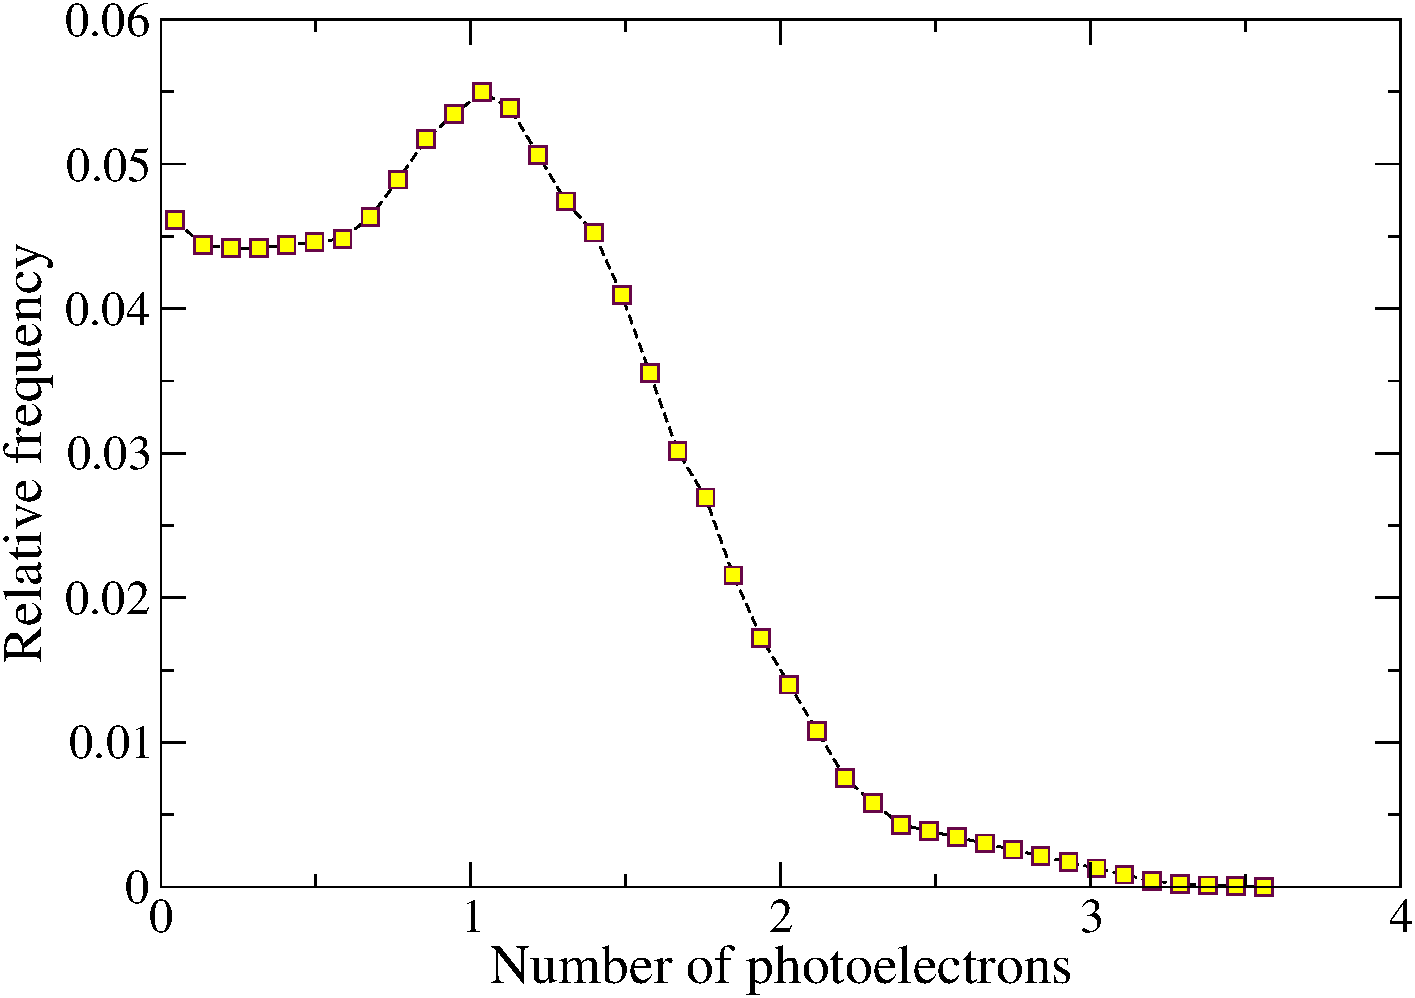
\includegraphics[width=.6\textwidth]{sps}
  \caption{Normalized Single Photoelectron Spectrum, as used by 
    the program \camera}
  \label{fig:sps}
\end{figure}



\section{Event Display}
\label{sec:eventdisplay}

A small program was developed for private use, for the display of the
events. In Fig. \ref{fig:qmagicdisplay} there is an example of such
program running. A $500\u{GeV}$ gamma initiated shower image is shown.

\begin{figure}[htbp]
  \centering
  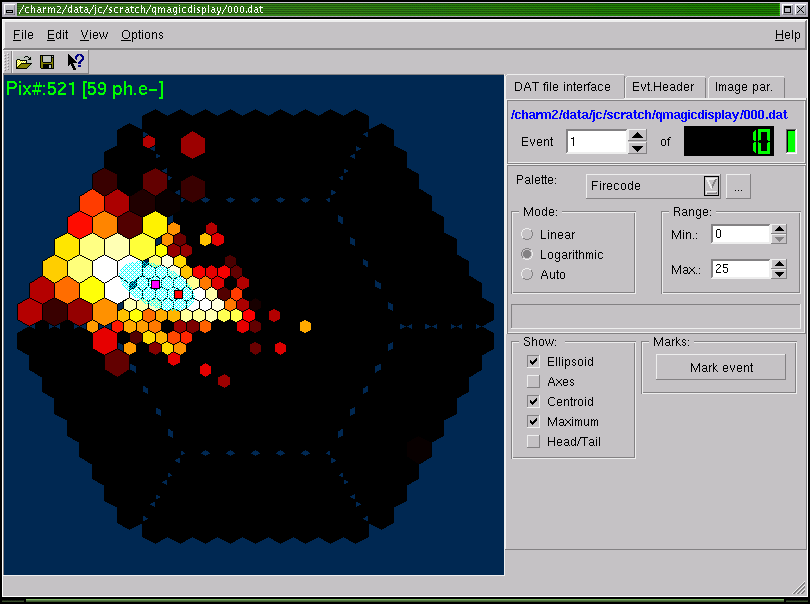
\includegraphics[width=\textwidth]{qmagicdisplay1}
  \caption{A gamma initiated shower image, with $500\u{GeV}$ as primary
    energy, displayed with the event display created for \MAGIC \MC
    data.}
  \label{fig:qmagicdisplay}
\end{figure}


\endinput
%
%% Local Variables:
%% mode:latex
%% TeX-master: t
%% End:

%%EOF
